Appendix \ref{sec:figures} contains Figures and Tables that are not specific to the project, but were referred to in the dissertation.

\begin{figure}[h]
	\centering
	\begin{subfigure}[b]{\textwidth}
		\centering
		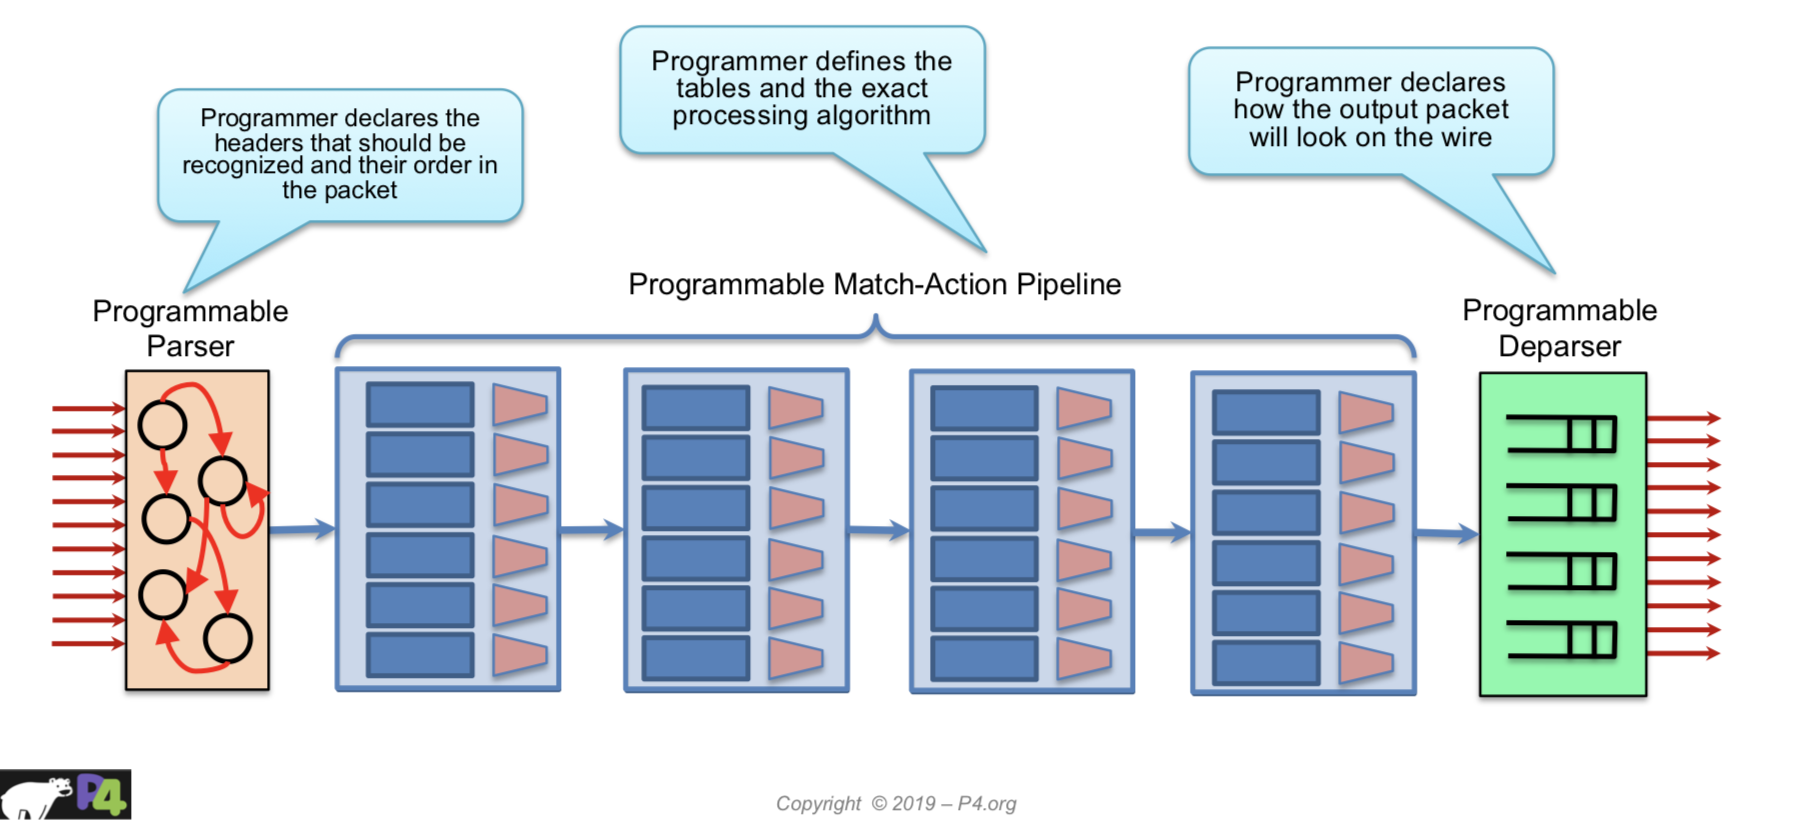
\includegraphics[width=\textwidth]{pisa.png}
		\caption{The single programmable pipeline forwarding architecture of PISA.}
		\label{fig:pisa}
	\end{subfigure}
	
	\vspace*{5mm}
	
	\begin{subfigure}[b]{\textwidth}
		\centering
		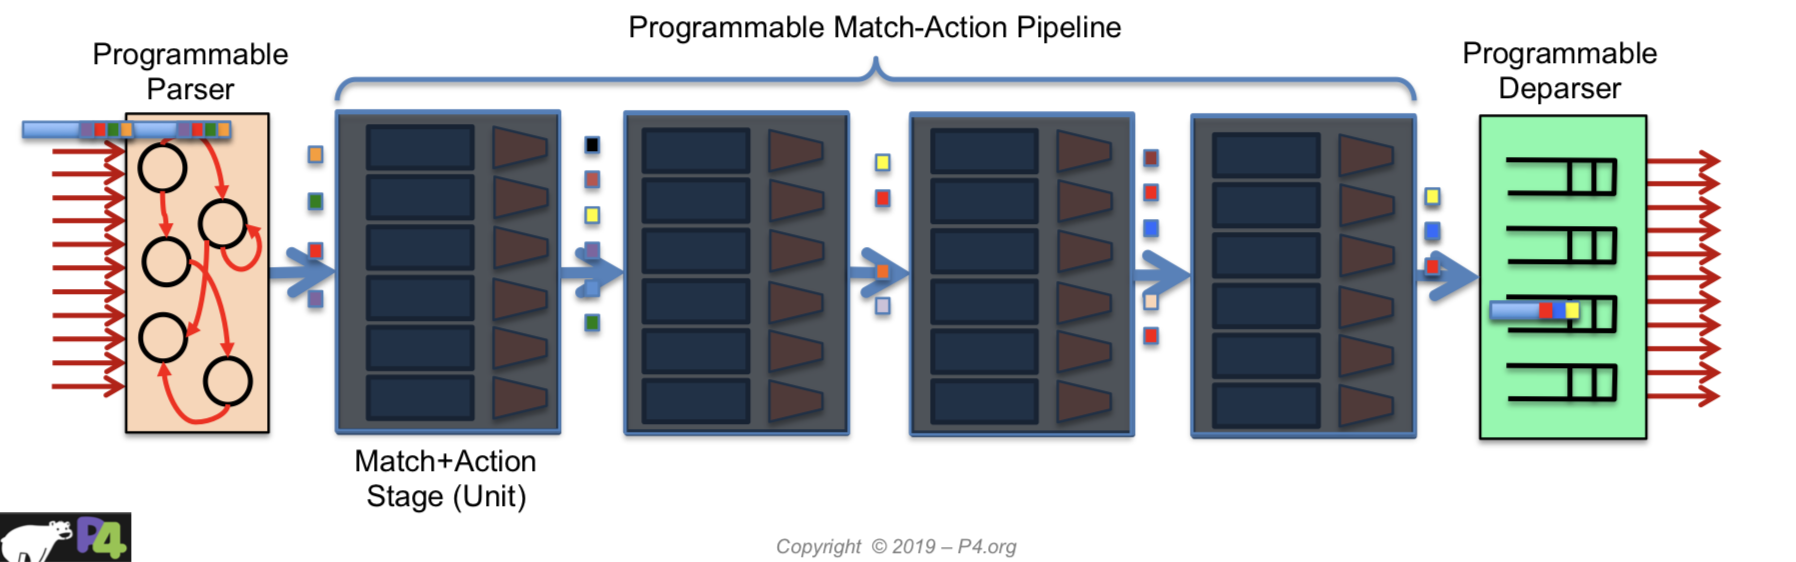
\includegraphics[width=\textwidth]{pisa1.png}
		\caption{The life cycle of a packet going through the PISA pipeline.}
		\label{fig:pisa1}
	\end{subfigure}
	\caption{PISA---Protocol-Independent Switch Architecture. Source: \href{https://p4.org}{P4.org -- Copyright \textcopyright\ 2019}.}
\end{figure}

\begin{table}[!ht]
	\begin{center}
		\caption{The P4$\rightarrow$NetFPGA extern functions library.}
		\label{tab:externs}
		\begin{tabular}{ | c | c | }
			\hline
			\multicolumn{2}{|c|}{\textbf{Stateful Atomic Extern Functions}} \\ \hline
			\textbf{Type} & \textbf{Description}  \\ \hline
			RW & Read or write state \\ \hline
			RAW & Read, add to, or overwrite state  \\ \hline
			PRAW & Either perform RAW or do not perform RAW based on predicate \\ \hline
			ifElseRAW & Two RAWs, one each for when a predicate is true or false \\ \hline
			Sub & IfElseRAW with stateful subtraction capability \\ \hline
			
			\multicolumn{2}{|c|}{\textbf{Stateless Extern Functions}} \\ \hline
			\textbf{Type} & \textbf{Description}  \\ \hline
			IP Checksum & Given an IP header, compute the IP checksum \\ \hline
			LRC & Longitudinal redundancy check, simple hash function \\ \hline
			timestamp & Generate timestamp (measured in clock cycles, granularity of 5ns) \\ \hline
		\end{tabular}
	\end{center}
\end{table}

\begin{figure}[!h]
	\centering
	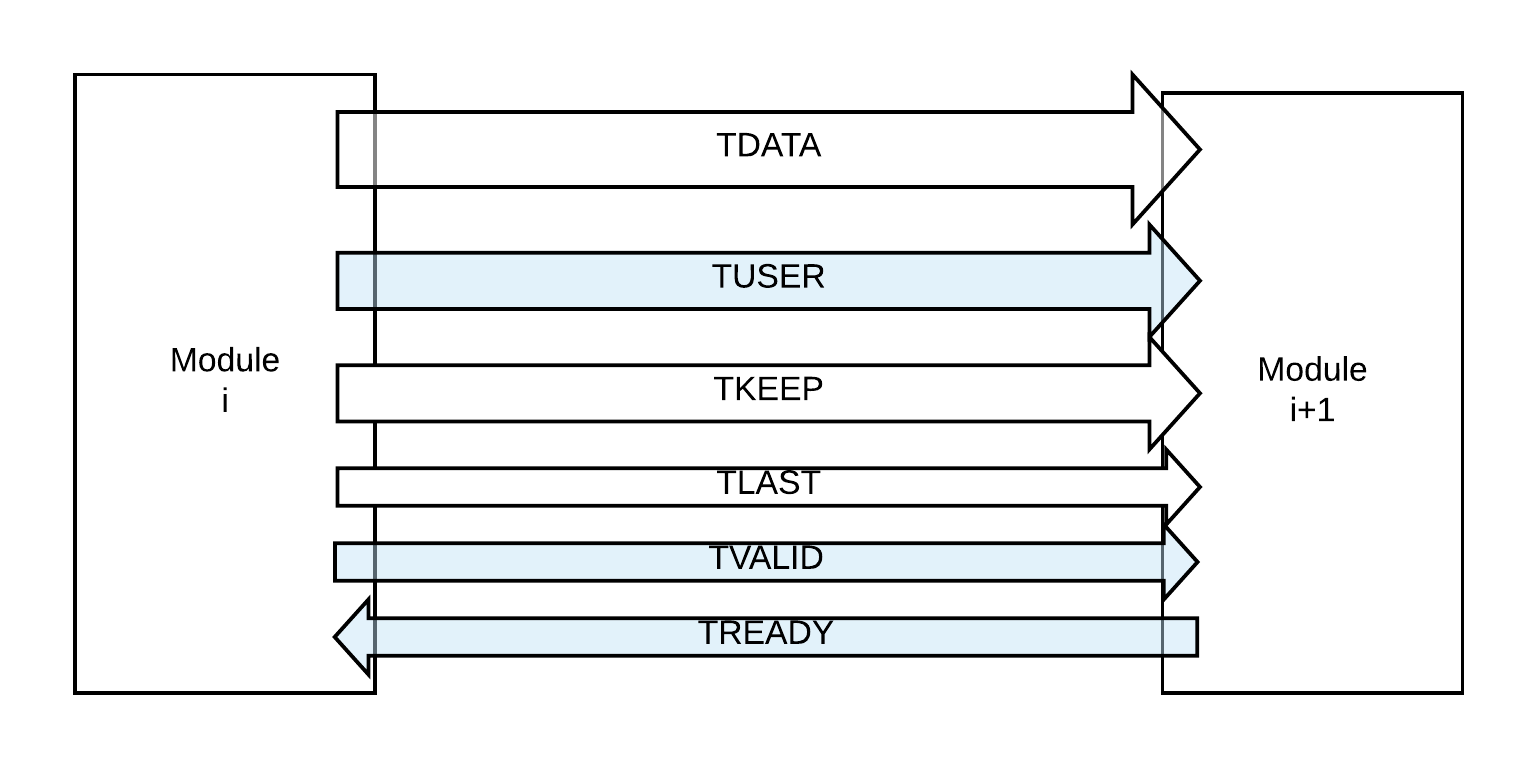
\includegraphics[width=0.85\textwidth]{axi.png}
	\caption{Inter-module communication is done via AXI-4 streams (Packets are moved as stream).}
	\label{fig:axi}
\end{figure}

\begin{table}[!h]
	\centering
	\caption{The AXI-4 streams and their descriptions.}
	\label{tab:axi}
	\begin{tabular}{ | l | l |}
		\hline
		\textbf{AXI-4 Stream} & \textbf{Description} \\ \hline
		TDATA & Data stream \\ \hline
		TKEEP & Marks NULL bytes (i.e. byte enable) \\ \hline
		TVALID & Validity indication \\ \hline
		TREADY & Flow control indication \\ \hline
		TLAST & End of packet/burst indication \\ \hline
		TUSER & Sideband metadata \\ \hline
	\end{tabular}
\end{table}